\documentclass[spanish,notitlepage,letterpaper, 12pt]{article} 
\usepackage[spanish]{babel} 
\usepackage{amsmath}
\usepackage{amsfonts}
\usepackage{amssymb}
\usepackage{graphicx}
\usepackage{geometry}      
\geometry{letterpaper}                  
\usepackage{epstopdf}
\usepackage{fancyhdr} % Paquete para encabezados y pies de pag
\usepackage{listings}
\usepackage{color}
\usepackage{placeins}
\usepackage{csquotes}
\usepackage{gensymb} 

\definecolor{dkgreen}{rgb}{0,0.6,0}
\definecolor{gray}{rgb}{0.5,0.5,0.5}
\definecolor{mauve}{rgb}{0.58,0,0.82}

\lstset{frame=shadowbox,
  language=Java,
  aboveskip=3mm,
  belowskip=3mm,
  showstringspaces=false,
  columns=flexible,
  basicstyle={\small\ttfamily},
  numbers=left,
  numberstyle=\tiny\color{gray},
  keywordstyle=\color{blue},
  commentstyle=\color{dkgreen},
  stringstyle=\color{mauve},
  breaklines=true,
  breakatwhitespace=true
  tabsize=3
  rulesepcolor=\color{blue}
}

\pagestyle{fancy} 
\chead{\bfseries Informe 1 - Grupo C1B. Subgrupo 2} 
\rhead{14 de Abril de 2023}
\cfoot{Universidad Industrial de Santander} 
\rfoot{\thepage} 

\voffset = -0.25in 
\textheight = 8.0in 
\textwidth = 6.5in
\oddsidemargin = 0.in
\headheight = 20pt 
\headwidth = 6.5in
\renewcommand{\headrulewidth}{0.5pt}
\renewcommand{\footrulewidth}{0,5pt}
\begin{document}
\begin{titlepage}
    \begin{center}
        
\includegraphics[width=0.4\textwidth]{../general-images/uis-logo.png}
        
        \vspace{0.5cm}
        \LARGE
        \textbf{Estudio del comportamiento del circuito RLC y el fenómeno de resonancia}
        
        \vspace{0.5cm}
        \large
        Informe 4
        
        \vfill
        
        \textbf{Daniel Esteban Vargas Reyes.} Estudiante - Geología\\
        \textbf{Nicolás Andrés Ramírez Calderón.} Estudiante - Ingeniería de Sistemas\\ 
        \textbf{Rodolfo Valentín Muñoz Vega.} Estudiante - Ingeniería Química\\

        \vspace{1.0cm}
        Presentado a la docente:
        
        \textbf{Zayda Paola Reyes Quijano}
        
        \vfill
        
        Escuela de Física - Física III\\
        Universidad Industrial de Santander\\
        Bucaramanga, Santander, Colombia\\
        20 de Mayo de 2023        
    \end{center}
\end{titlepage}

\tableofcontents

\newpage

\section{Resumen}
Para el siguiente informe se busca explicar de manera clara el desarrollo de la práctica de laboratorio “Estudio del MAS del péndulo simple y péndulo reversible”; la cual discierne en la toma de datos para encontrar el valor de la gravedad para luego tener en cuenta el error que se produce al momento de realizar el proceso experimental. Además, se pretenden afianzar los conocimientos del movimiento armónico simple y sus connotaciones teórico-prácticas que son determinantes para tomar conclusiones acertadas.  

\section{Introducción}
Varios de los fenómenos cotidianos que solemos catalogar como \enquote{abstractos} guardan una profunda similitud con el comportamiento de objetos como los péndulo. La física nos permite comprender estos sucesos en aras de obtener avances para nuestra sociedad.\\

El movimiento armónico simple se define como aquel en el que la aceleración del objeto es siempre proporcional a su posición y en dirección opuesta al desplazamiento del punto de equilibrio. \cite{serway_jewett_2017}\\

En este proyecto se pretende estudiar el MAS (Movimiento Armónico Simple) del péndulo simple y del péndulo reversible, para ello se requiere analizar el periodo de oscilación de los péndulos, su longitud al centro de masa y la relación de estas variables con la gravedad.\\

\subsection{Marco teórico} \label{I.MT}
\subsubsection{Péndulo simple}
Este tipo de péndulo es aquel que presenta condiciones ideales; sin fricción y con la masa concentrada en un solo punto. Consta de una masa puntual atada a una cuerda de longitud $L$ carente de masa. (Fig. \ref{Figura 1}) 

\begin{figure}[h]
    \centering
    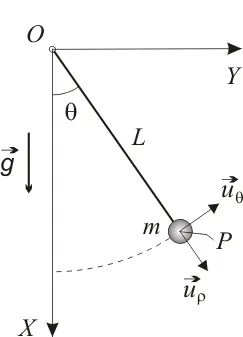
\includegraphics[width=4.0cm]{images/Pendulo-simple.png}
    \caption{Péndulo simple}
    \label{Figura 1}
\end{figure}
    
Si se relaciona la fuerza recuperadora del sistema, que en esencia proviene del peso, con la segunda ley de Newton, se tiene que: 
\begin{equation}
    ma=-mg\sin{\theta}
\end{equation}
Realizando algunas sustituciones y teniendo en cuenta que la frecuencia $w²=\frac{g}{L}$ la ecuación puede escribirse de la forma:
\begin{equation}
    \frac{d^2\theta}{dt^2}L=-g\sin{\theta}
\end{equation}
Es visible que la oscilación descrita realmente no se trata de un MAS. Sin embargo, para cierto rango de valores para $\theta$ se tiene que $\sin{\theta}\approx\theta$, en cuyo caso si sería un MAS. El rango mencionado no está formalmente definido, pero para este caso utilizamos $\theta<15\degree$.
\begin{equation}
    \frac{d^2\theta}{dt^2}=-\frac{g}{L}\theta
\end{equation}
La función $\theta(t)$ que soluciona la ecuación diferencial tiene la forma:
\begin{equation}
    \theta(t)=\theta_0\cos{(\omega t+\varphi)}
\end{equation}
Donde $\theta_0$ es la amplitud del movimiento oscilatorio (el ángulo inicial desde el que fue soltada la masa), $\omega$ la frecuencia y $\varphi$ el desfase. \cite{serway_jewett_2017}\\

Por otra parte, es posible expresar el periodo teniendo en cuenta el valor de la frecuencia angular $\omega$ de la forma:
\begin{equation}
    T=\frac{2\pi}{\omega}=2\pi\sqrt{\frac{L}{g}}
\end{equation}

\subsubsection{Péndulo compuesto}
\quote{Si un objeto colgante oscila sobre un eje fijo que no pasa a través de su centro de masa y el objeto no puede aproximarse como una masa puntual, entonces ya no se trata de un péndulo simple. En este caso se habla de un \textbf{péndulo físico} (o compuesto).} \cite{serway_jewett_2017}\\

\begin{figure}[h]
    \centering
    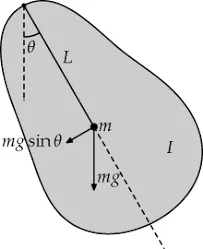
\includegraphics[width=4.0cm]{images/Pendulo-compuesto.png}
    \caption{Péndulo compuesto}
    \label{Figura 2}
\end{figure}

Si se considera un cuerpo que oscila al rededor de un eje a una distancia $L$ del centro de masa (Fig. \ref{Figura 2}), la gravedad proporciona un torque sobre el eje de giro. De modo que utilizando la forma rotacional de de la segunda ley de Newton se tiene que:
\begin{equation}
    -mgL\sin{\theta}=I\frac{d^2\theta}{dt^2}
\end{equation}
Donde $I$ es el momento de inercia del cuerpo con respecto al eje de giro.\\

Ya se conoce que para ángulos pequeños $\theta\approx\sin{\theta}$, luego:
\begin{equation}
    \frac{d^2\theta}{dt^2}=-\frac{mgL}{I}\theta=-\omega^2\theta
\end{equation}
De la cual se puede deducir que la frecuencia $\omega$ es:
\begin{equation}
    \omega=\sqrt{\frac{mgL}{I}}
\end{equation}
Y el periodo $T$:
\begin{equation}
    T=\frac{2\pi}{\omega}=2\pi\sqrt{\frac{I}{mgL}}
\end{equation}
No obstante, gracias al teorema de los ejes paralelos \cite{serway_jewett_2017} es posible expresar esta ecuación en términos del momento de inercia del centro de masa y simplificarla de la siguiente forma:
\begin{equation}
    I=I_{CM}+mh^2=m(h^2+K^2)
\end{equation}
Donde $I_{CM}$ es el momento de inercia respecto al centro de masa y $K$ es el radio de giro. Luego el periodo queda:
\begin{equation}
    T=2\pi\sqrt{\frac{h^2+K^2}{gh}}
\end{equation}

Para este experimento se utilizó un péndulo de Kater (también llamado péndulo reversible) que es un caso del péndulo compuesto con dos puntos de suspensión $H_1$ y $H_2$ y con masas desplazables para conseguir periodos de oscilación iguales alrededor de ambos bordes. Para este caso la longitud reducida del péndulo es igual a la distancia entre los
bordes $d=99.4cm$.\\

Para el péndulo reversible puesto a punto, se tiene que se puede obtener el valor de la
aceleración de la gravedad a partir de:
\begin{equation}
    \label{eq:12}
    g=4\pi^2\frac{d}{T^2}
\end{equation}
\section{Metodología}
El desarrollo del experimento se realizó en tres etapas; dos de recolección de datos y una de análisis, pero previo a la explicación de estas etapas es importante detallar los materiales utilizados para esta práctica:
\subsection{Materiales}
\begin{enumerate}
    \item Péndulo simple
    \item Péndulo reversible
    \item Base
    \item Cinta métrica
    \item Cronómetro
\end{enumerate}
\subsection{Fase 1}
En esta fase se registrarán los datos para la obtención del período del péndulo reversible. Antes de iniciar la parte experimental, se realizó el montaje de la figura 1 (Fig. \ref{Figura 3}). La masa $m_1$ se ajustó en una posición fija respecto al punto de suspensión $H_1$. Luego se ajustó la distancia $x_1$, que es la distancia comprendida desde $H_1$ hasta la masa $m_1$. Después, se separaró el péndulo de su posición de equilibrio un ángulo pequeño y se registró el tiempo $t$ de $10$ oscilaciones. Este procedimiento se realizó para diferentes distancias $x_2$.
Luego de ello, se invirtió la posición del péndulo cambiando el eje de suspensión a
$H_2$ y se repitió el procedimiento anterior registrando los tiempos $t\prime$ de 10 oscilaciones. Con los valores de los promedios de los tiempos $t$ y $t\prime$ se determinararon los
períodos $T$ y $T\prime$.
\begin{figure}[h]
    \centering
    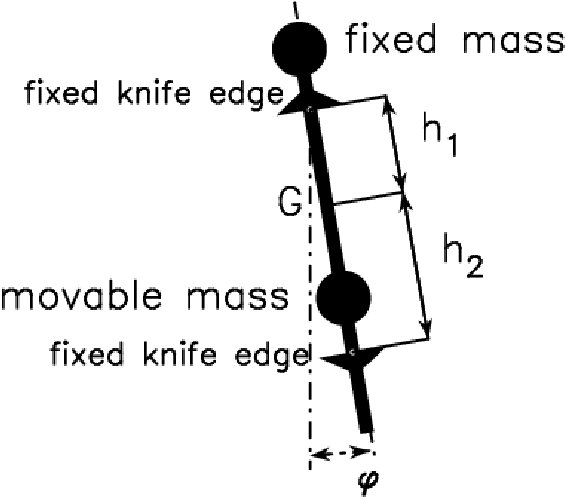
\includegraphics[width=10.0cm]{images/Pendulo-Kater.png}
    \caption{Péndulo de Kater}
    \label{Figura 3}
\end{figure}
\subsection{Fase 2}
En esta fase se obtuvieron los datos para el análisis del período del péndulo simple y la obtención de la aceleración de la gravedad. Para ello, se utilizó péndulo simple de longitud L, sujetando una masa a un hilo inextensible. Se registraron los tiempos de diez oscilaciones para siete longitudes. Por último, se calculó el periodo $\bar{T}$, $\bar{T}^2$.
\subsection{Fase 3}
En esta fase se analizó la dependencia del período de oscilación de un
péndulo reversible con la distancia $x_2$ y la dependencia del período del péndulo simple
con su longitud. En el caso del péndulo reversible (fase uno), se realizó un gráfico $\bar{T}^2$ y $\bar{T\prime}^2$ como funciones de $x_2$. Luego se realizó un análisis
gráfico, determinando las ecuaciones de las funciones. Luego se determinaron los puntos de intersección de las dos gráficas, los valores de $\bar{T}^2$ y $\bar{T\prime}^2$ para éstos puntos y se calculó el valor promedio $T_{prom}^2$.\\

Además, asumiendo un valor $d=0.99m$ se encontró el valor experimental de la gravedad a partir de la expresión encontrada previamente en la sección \ref{I.MT} \eqref{eq:12}. Para este caso se reemplazó el $T^2$ por el $T_{prom}^2$.\\

Por último, se repitió el cálculo anterior asumiendo $d=d_1+d_2$ (suma de los
interceptos correspondientes a la coordenada $x_2$.
\section{Tratamiento de datos} \label{TD}
El laboratorio inicialmente se dividió en dos fases importantes. La FASE 1, donde se analizan las oscilaciones armónicas de un péndulo reversible. Por otra parte, en la FASE 2, se analizará la dependencia del período de oscilación de un péndulo simple.
\subsection{Fase 1} \label{TD.Fase1}
Para esta fase se realizo la toma de datos suficientes para lograr los promedios más específicos y evitar la mayor cantidad de errores. Se tomaron datos de tiempo respecto a 10 oscilaciones. Los datos de esta fase se ven en la tabla (cdr. \ref{Table 1}).
\newpage
\begin{table}[h]
    \centering
    \begin{tabular}{l|c|c|c|c|c|c|c|c|c|l}
        $x_2 \ [m]$ & $t_1 \ [s]$ & $t_2 \ [s]$ & $t_3 \ [s]$ & $\bar{T} \ [s]$ & $\bar{T}^2 \ [s^2]$ & $t_1 \ [s]$ & $t_2 \ [s]$ & $t_3 \ [s]$ & $\bar{T}\prime \ [s]$ & ${\bar{T}\prime}^2 \ [s^2]$   \\
        \hline \hline
        $0.015$ & $20.71$ & $20.81$ & $20.89$ & $2.08$ & $4.33$ & $21.04$ & $20.98$ & $20.97$ & $2.09$ & $4.41$ \\
        $0.030$ & $20.24$ & $19.98$ & $20.01$ & $2.01$ & $4.03$ & $20.18$ & $20.29$ & $20.36$ & $2.03$ & $4.10$ \\
        $0.045$ & $19.62$ & $19.97$ & $19.93$ & $1.98$ & $3.93$ & $19.85$ & $19.80$ & $19.91$ & $1.98$ & $3.94$ \\
        $0.060$ & $19.74$ & $19.81$ & $19.77$ & $1.98$ & $3.91$ & $20.03$ & $19.93$ & $20.11$ & $2.00$ & $4.01$ \\
        $0.075$ & $19.97$ & $20.02$ & $20.05$ & $2.005$ & $4.01$ & $21.13$ & $21.02$ & $21.09$ & $2.11$ & $4.44$ \\
        $0.090$ & $20.48$ & $20.61$ & $20.64$ & $2.06$ & $4.23$ & $24.40$ & $24.54$ & $24.74$ & $2.46$ & $6.04$
    \end{tabular}
    \caption{Tiempos y periodos de oscilaciones armónicas de un péndulo reversible}
    \label{Table 1}
\end{table}

Luego de tomar meticulosamente los datos, se realizan las gráficas correspondientes de los periodos al cuadrado ($T^2$ y ${T\prime}^2$) contra la longitud o distancia tomadas respecto al centro de masa de la barra ($x_2$). La grafica se muestra en la figura (fig. \ref{Figura 4})
\begin{figure}[h]
    \centering
    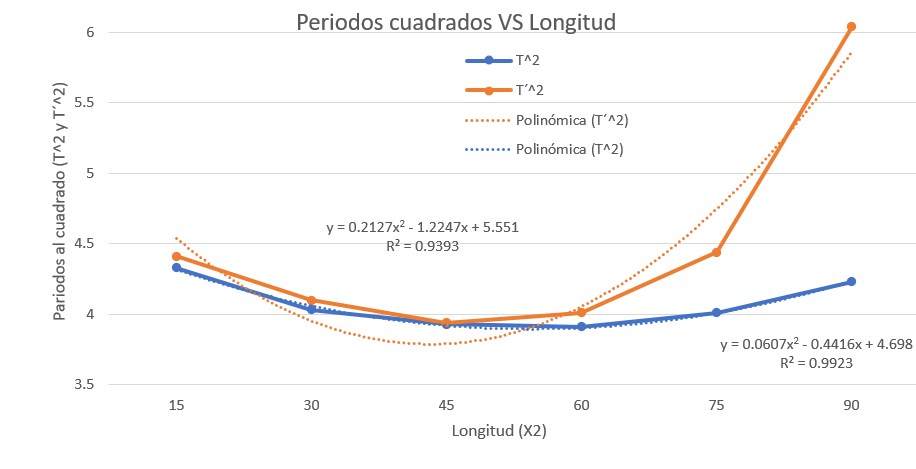
\includegraphics[width=15.0cm]{images/Periodos-cuadrados.png}
    \caption{Gráfica de los periodos cuadrados vs longitud}
    \label{Figura 4}
\end{figure}

Para la grafica de la figura anterior (fig. \ref{Figura 4}), se usaron los datos $x_2$, $T^2$ y ${T\prime}^2$ tabla (cdr. \ref{Table 1}). Además, se hizo uso de la ecuación de la gravedad expuesta en la sección \ref{I.MT} \eqref{eq:12} donde $d=x_1+x_2$ cuando $x_1$ y $x_2$ son los puntos entre las curvas de la figura previa (fig. \ref{Figura 1}). Para encontrar estos puntos se igualaron las ecuaciones de las curvas y posteriormente encontrando el valor de la variable mediante la fórmula cuadrática.
\begin{equation}
    0.0607x^2-0.4416x+4.698=0.2127x^2-1.2247x+5.551
\end{equation}
\begin{equation}
    -0.152x^2+0.7831x-0.853=0\\
\end{equation}
Donde resultaron las siguientes raices.

\begin{equation}
    x_1=\frac{0.7831\pm\sqrt{0.09462161}}{0.304}
\end{equation}

Tomando los valores de $x_1=1.56$ y $x_2=3.59$ el valor de $d$ pasa a ser $d=1.56$ y $d_3.59$ respectivamente. En este caso se utilizará $x_1$ ya que es el que mejor se acerca al valor de la gravedad.\\

Para el valor de $T_{prom}$ se utilizan los valores de $T_2=4.07$ y $T\prime²=4.49$ sabiendo que estos son los valores promediados de los periodos tomados anteriormente. (cdr. \ref{Table 1}) $$T_{prom}=4.28$$
Ahora se reemplazan los datos de $d$ y $T_{prom}$ en la ecuación de la gravedad obteniendo: $$G=12.9 \ \frac{m}{s²}$$
Para encontrar el porcentaje de error del proceeso experimental se utiliza la siguiente fórmula: $$\%e=\frac{V_e-V_t}{V_t}\cdot100$$ En este caso se utiliza el valor real de la gravedad como valor teórico: $$\%e=31.6\%$$
\subsection{Fase 2}
Para esta fase se tomaron datos similares a los de la sección \ref{TD.Fase1}, tomando de referencia $10$ oscilaciones y teniendo en cuenta el dato del tiempo, notando que en este caso se varía la longitud de la cuerda. Los datos de la fase se presentan en la siguiente tabla (cdr. \ref{Table 2}).

\begin{table}[h]
    \centering
    \begin{tabular}{l|c|c|c|c|c|l}
        $L \ [m]$ & $t_1 \ [s]$ & $t_2 \ [s]$ & $t_3 \ [s]$ & $\bar{t} \ [s]$ & $\bar{T}=\frac{\bar{t}}{N} \ [s]$ & $\bar{T}^2 \ [s^2]$   \\
        \hline \hline
        $0.015$ & $7.36$ & $7.39$ & $7.47$ & $7.41$ & $0.71$ & $0.50$\\
        $0.020$ & $8.84$ & $8.87$ & $9.02$ & $8.77$ & $1.22$ & $1.49$\\
        $0.026$ & $10.15$ & $10.14$ & $10.36$ & $10.22$ & $1.02$ & $1.04$\\
        $0.030$ & $10.74$ & $10.82$ & $10.95$ & $10.84$ & $1.08$ & $1.18$\\
        $0.036$ & $11.81$ & $11.75$ & $11.80$ & $11.79$ & $1.18$ & $1.39$\\
        $0.040$ & $12.33$ & $12.35$ & $13.69$ & $12.79$ & $1.28$ & $1.64$\\
        $0.046$ & $13.40$ & $13.33$ & $13.39$ & $13.37$ & $1.34$ & $1.79$\\
    \end{tabular}
    \caption{Dependencia del periodo de oscilación de un péndulo simple}
    \label{Table 2}
\end{table}

Luego de la toma de datos, se procedió a realizar la gráfica en la que se representan los valores de $T^2$ contra los valores de longitud de la cuerda $L$. La grafica se muestra en la siguiente figura (fig. \ref{Figura 5}).
\newpage
\begin{figure}[h]
    \centering
    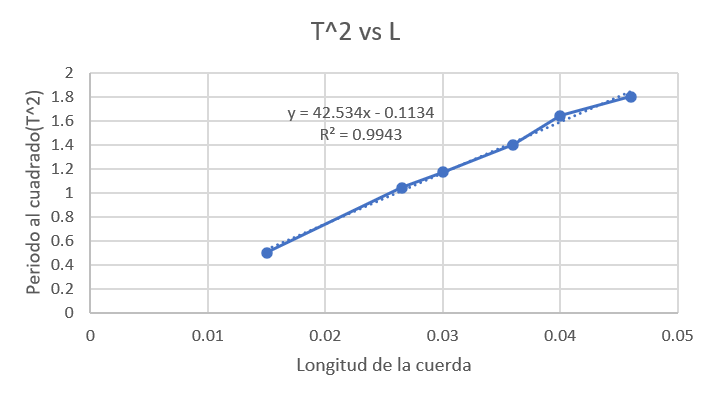
\includegraphics[width=15.0cm]{images/pc-vs-lc.png}
    \caption{Gráfica de periodos cuadrados vs longitud de cuerda}
    \label{Figura 5}
\end{figure}

Para el análisis de los datos presentados inicialmente nos basamos en la fómula de la función lineal:
\begin{equation} \label{eq:21}
    y=mx+b
\end{equation}
Como se pretende encontrar el valor experimental de la gravedad usamos la ecuación anterior \eqref{eq:21} como base, para luego despejar la gravedad.
\begin{equation} \label{eq:22}
    T=2\pi\sqrt{\frac{L}{g}}
\end{equation}
Como se graficó el periodo al cuadrado buscamos poner la fórmula \eqref{eq:22} en orden de estos términos elevando al cuadrado la función, y quedó de la siguiente forma:
\begin{equation} \label{eq:23}
    T^2=4\pi^2\frac{L}{g}
\end{equation}
La ecuación \eqref{eq:23} ya está de la forma \eqref{eq:21} , donde $y=T^2$ y $x=L$. Como los valores ya se encuentran graficados con sus respectivos ejes, la pendiente sería:
\begin{equation} 
    m=\frac{4\pi^2}{g}
\end{equation}
Función de la cual se despeja la gravedad para notar que esta queda en términos de la pendiente; para conocer este valor nos basamos en la recta mostrada en la figura (fig. \ref{Figura 5}) donde $m=$. Reemplazando para hallar la gravedad:
\begin{equation}
    g=0.92 \ [\frac{m}{s^2}]
\end{equation}
Para encontrar el porcentaje de error se aplica el mismo proceso que en la sección \ref{TD.Fase1}: $$\%e=90.8\%$$

\section{Análisis de resultados}

Inicialmente los resultados esperados por parte del equipo de trabajo eran que a medida que se cambiara la longitud del péndulo físico o del péndulo simple, el periodo variaría en función de dicha longitud, solo que no se tenía certeza de que tipo de variación sería, pero teniendo en cuenta que si la longitud del péndulo tiende a 0, así tambien será el periodo. Además, con lo mostrado en la sección \ref{TD}, se puede discutir sobre los resultados, haciendo un contraste entre los resultados esperados y los obtenidos.\\

Se puede observar en las tablas revias (cdr. \ref{Table 1}, \ref{Table 2}) los resultados obtenidos mediante el proceso de experimentación y en ambos casos se observa que el periodo tiene un comportamiento de una función cuadrática, “como se esperaba”, más sin embargo los resultados experimentales podrían diferir con los esperados puesto a que entra la variable del porcentaje de error, que afecta en la medición de cada una de las variables físicas que interfieren en el péndulo, tales como la toma de la longitud, la toma del ángulo y el conteo de las oscilaciones que no fueron extremadamente exactas. Lo anterior afecta de forma directa los resultados obtenidos.
\section{Conclusiones}
Cerrando con el proceso de experimentación y de investigación se pudieron cumplir los objetivos y se obtuvo el entendimiento necesario para captar los fenómenos físicos que intervienen en el  péndulo reversible y el péndulo simple. Por otra parte, con los resultados que se tenían previstos obtener “resultados esperados”, se realizó una comparación demostrando que había cierto margen de error, pero dicho error era en cierta medida despreciable, ya que se debe al error del “factor humano”, tal como en la toma de los tiempos y toma de ángulos, además se pudo entender el funcionamiento físico de ambos péndulos. En el análisis de datos también se pudo observar que la línea de tendencia que describe el péndulo reversible es cuadrática, explicando su comportamiento a medida que avanza el tiempo, mientras que, en el péndulo simple, su línea de tendencia análizando el periodo cuadrado describe la función lineal \eqref{eq:21}.

\section{Referencias} 
\bibliographystyle{unsrt}
\bibliography{../general-references/references}
\end{document}
